\documentclass[11pt]{article}

%% \usepackage{amsmath,amssymb,amsthm}
\usepackage{hyperref}
\usepackage[usenames]{color}
\usepackage[margin=1in]{geometry}
\usepackage{graphicx}
\usepackage{subfigure}
\usepackage[round, semicolon]{natbib}
%%\usepackage[round,colon]{natbib}

% \newcommand{\todovk}[1]{{\marginpar{\color{blue} (VK) #1}}}
% \newcommand{\todoea}[1]{{\marginpar{\color{red} (EA) #1}}}
% \newcommand{\vknote}[1]{{\color{blue} (VK) #1}}
% \newcommand{\eanote}[1]{{\color{red} (EA) #1}}
\newcommand{\todovk}[1]{}
\newcommand{\todoea}[1]{}
% \newcommand{\vknote}[1]{{\color{blue} (VK) #1}}
% \newcommand{\eanote}[1]{{\color{red} (EA) #1}}
\newcommand{\eat}[1]{ }

\def\ie{{\it i.e.},~}
\def\eg{{\it e.g.},~}
\def\etal{{\it et al.}~}

\def\NP{\mathsf{NP}}
\def\RP{\mathsf{RP}}
\def\bnsel{\mathsf{BN\mbox{-}Sel}}
\def\optsel{\mathsf{Opt\mbox{-}Sel}}
\def\NZ{\mathsf{NZ}}
\def\sparsity{\mathrm{sparsity}}
\def\scA{{\mathcal A}}
\def\scG{{\mathcal G}}
\def\EX{\mathsf{EX}}
\def\E{\mathbb{E}}
\def\moo{{\{-1, 1\}}}
\def\reals{\mathbb{R}}
\def\one{\mathds{1}}
\def\OS{\mathsf{OS}}
\def\OU{\mathsf{OU}}
\def\PAC{\mathsf{PAC}}
\def\junta{{\mathcal J}}
\def\Poisson{\mathrm{Poisson}}
\def\yy{{\mathcal Y}}
\def\poly{\mathrm{poly}}
\def\Nu{{\mathcal V}}
\def\transpose{T}
\def\th{{^{\textit{th}}}}
\def\lerr{\mathrm{\ell_2\mbox{-}err}}
\def\wmin{w_{\mbox{\footnotesize{min}}}}
\def\wmax{w_{\mbox{\footnotesize{max}}}}
\def\corr{\mathrm{corr}}
\def\argmin{\mathrm{argmin}}
\def\var{\mathrm{var}}
\def\lerror{\mathrm{\ell_2\mbox{-}error}}
\def\sparseset{\mathrm{sparse\mbox{-}set}}
\def\Mut{\mathsf{Mut}}
\def\Neigh{\mathsf{Neigh}}
\def\naturals{\mathbb{N}}
\def\Bene{\mathsf{Bene}}
\def\Neut{\mathsf{Neut}}
\def\opt{\mathsf{opt}}
\def\best{\mathsf{Best}}
\def\evalg{{\mathcal EA}}
\def\Sel{\mathsf{Sel}}
\def\Dists{{\mathcal D}}
\def\loss{\mathrm{L}}
\def\lin{\mathsf{Lin}}

\newcommand{\dtv}[1]{{ \Vert #1 \Vert_{\mbox{\footnotesize{TV}}}}}
\newcommand{\pinorm}[1]{{ \Vert #1 \Vert_{\pi}}}
\newcommand{\lznorm}[1]{\mathrm{sparsity}(#1)}
\newcommand{\ltwonorm}[1]{\Vert #1 \Vert}
\newcommand{\ip}[2]{\langle #1, #2 \rangle}

\newtheorem{lemma}{Lemma}
\newtheorem{theorem}{Theorem}
\newtheorem{remark}{Remark}
\newtheorem{definition}{Definition}
\newtheorem{proposition}{Proposition}
\newtheorem{claim}{Claim}


\begin{document}
\title{Attribute-Efficient Evolvability of Linear Functions} 
\author{Elaine Angelino \\
Harvard University \\ \texttt{elaine@eecs.harvard.edu} \and Varun
Kanade \\ UC Berkeley \\ \texttt{vkanade@eecs.berkeley.edu}}

\maketitle

Darwin's theory of evolution through natural selection has been a cornerstone of
biology for over a century and a half.  Natural selection acts on
\emph{phenotypes} that are a result of molecular activities at the level of
cells; the molecular activities themselves are encoded in the DNA sequence, or
\emph{genotype}.\footnote{There are epigenetic factors at play, but the general
principle expounded in this document applies to those mechanisms as well.}
Every cell is a computing machine, sensing its environment and producing
appropriate responses.  Abstractly, cellular activity can be viewed as computing
a function; the input is an ``internal representation'' of the environment using
proteins and other molecules, and the output is the activation or repression
of proteins expression. Yet, a quantitative theory of the complexity of such
functions that could arise through Darwinian mechanisms has remained virtually
unexplored. Here, complexity is viewed through the lens of theoretical
computer science, \eg the size of the circuit required to compute the
function~\citep{Arora-Barak:textbook, Papadimitriou:textbook}.

To address this question, \citet{Valiant:2009-evolvability} introduced a
computational model of evolution.  In this model, an organism is an entity that
computes a function of its environment. For simplicity, each organism computes
only one function, though in reality there may be
thousands if not more. There is a (possibly hypothetical)
\emph{ideal function} indicating the best behavior in every possible
environment. The performance of the organism is measured by how close the
function it computes is to the ideal. An organism produces a set of offspring,
that may have mutations that  alter the function computed. The performance
(fitness) measure acting on a population of mutants forms the basis of natural
selection.\footnote{Recombination may increase the speed of evolution, but it is
understood that in Valiant's model, it does not affect the complexity that can
arise in functions.} The resources allowed are the most generous while remaining
feasible; the mutation mechanism may be any efficient randomized Turing
machine,\footnote{A Turing machine is a mathematical model on which all modern
computers are based; the widely believed Church-Turing hypothesis states that
\emph{any} feasible computation in nature can be simulated by a Turing
machine.} and the function represented by the organism may be arbitrary as long
as it is computable by an efficient Turing machine.

Formulated this way, the question of evolvability can be asked in the language
of computational learning theory. For what classes of ideal functions, $C$, can
one expect to find an evolutionary mechanism that gets arbitrarily close to the
ideal, within feasible computational resources? A function class captures a
notion of complexity, say for example,
%%
\[ f(x_1, \ldots, x_n) = 2 x_1 + 3.7 x_4 - 7.8 x_9 + 6 x_{12} + 18, \]
%%
is a linear function, and one could consider the class of all such linear
functions. A more complex class is that of quadratic functions, where a function
takes the form $f(x_1, \ldots, x_n) = 3.2 x_1^2 - 7.3 x_1 x_6 + 18 x_3 + 8.1$.
The point here is that the highest degree of any term appearing the expression
is $2$. One expects that the more \emph{complex} the ideal function, the harder
it is for evolution to succeed in approximating it.

Valiant's model is general in the sense that mutations are allowed to be
arbitrary and no explicit 




rather arbitrary and biologically unnatural.
Current understanding of biology (or lack thereof) makes it
difficult to formalize a notion of \emph{naturalness} for mutations in these
frameworks; in particular, it is not well understood how mutations to DNA
relate to functional changes in an organism. That said, the more direct
algorithms are appealing due to the simplicity of their mutations.  Also, the
``chemical computers'' of organisms may be slow, and hence, representations that
have low complexity are attractive.  In general, Feldman's
generic reduction from statistical query algorithms may use arbitrarily complex
representations (polynomial-sized circuits), depending on the specific algorithm
used.  In the remainder of the introduction, we first describe a particular
class of biological circuits, \emph{transcription networks}, that motivate our
study.  We then frame the evolutionary question in the language of computational
learning theory, summarize our contributions and discuss related work.

\subsection*{Representation in Biology}

Biological systems appear to function successfully with greatly restricted
representation classes. The nature of circuits found in biological systems may
vary, but some aspects -- such as \emph{sparsity} -- are common.  Specifically,
the interacting components in many biological circuits are sparsely connected.
Biological circuits are often represented as networks or graphs, where the
vertices correspond to entities such as neurons or molecules and the edges to
connections or interactions between pairs of entities. For example, both neural
networks~\cite{Watts:1998} and networks of metabolic reactions in the
cell~\cite{Wagner:2001,Barabasi:2000} have been described by ``small-world''
models, where a few ``hub'' nodes have many edges but most nodes have few edges
(and consequently, the corresponding graphs have small diameter).  An associated
property observed in biological networks is \emph{modularity}: a larger network
of interacting entities is composed of smaller modules of (functionally related)
entities~\cite{Hartwell:1999}.  Both the ``small-world'' description and
modularity of biological networks are consistent with the more general theme of
sparsity.

\begin{figure}[!t]
\centering
\subfigure[~]{
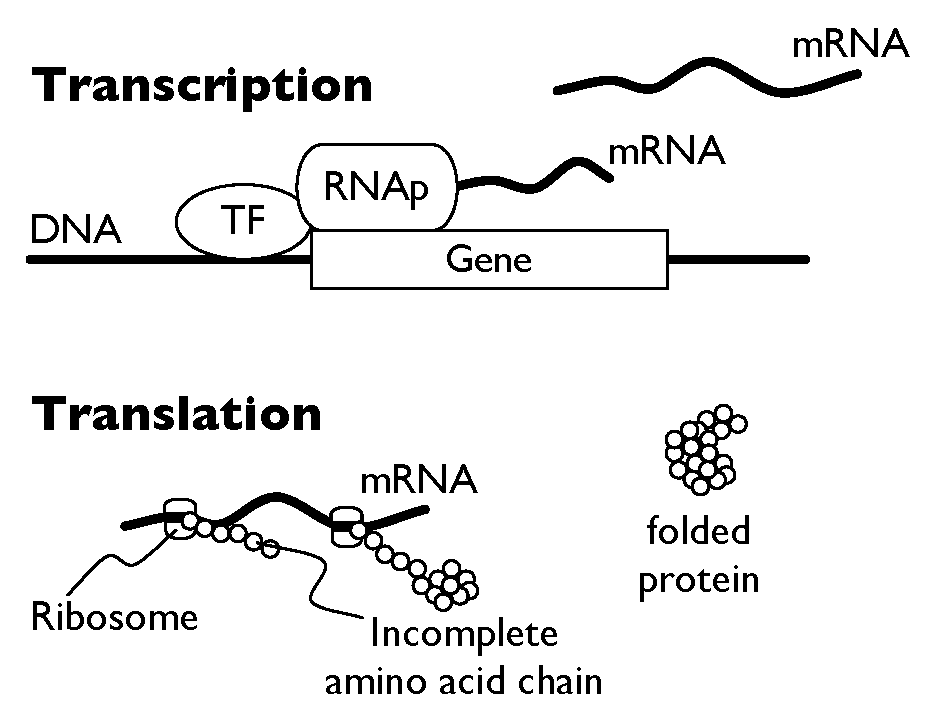
\includegraphics[width=0.47\textwidth]{figs/biology}
\label{fig:biology}
}
\subfigure[~]{
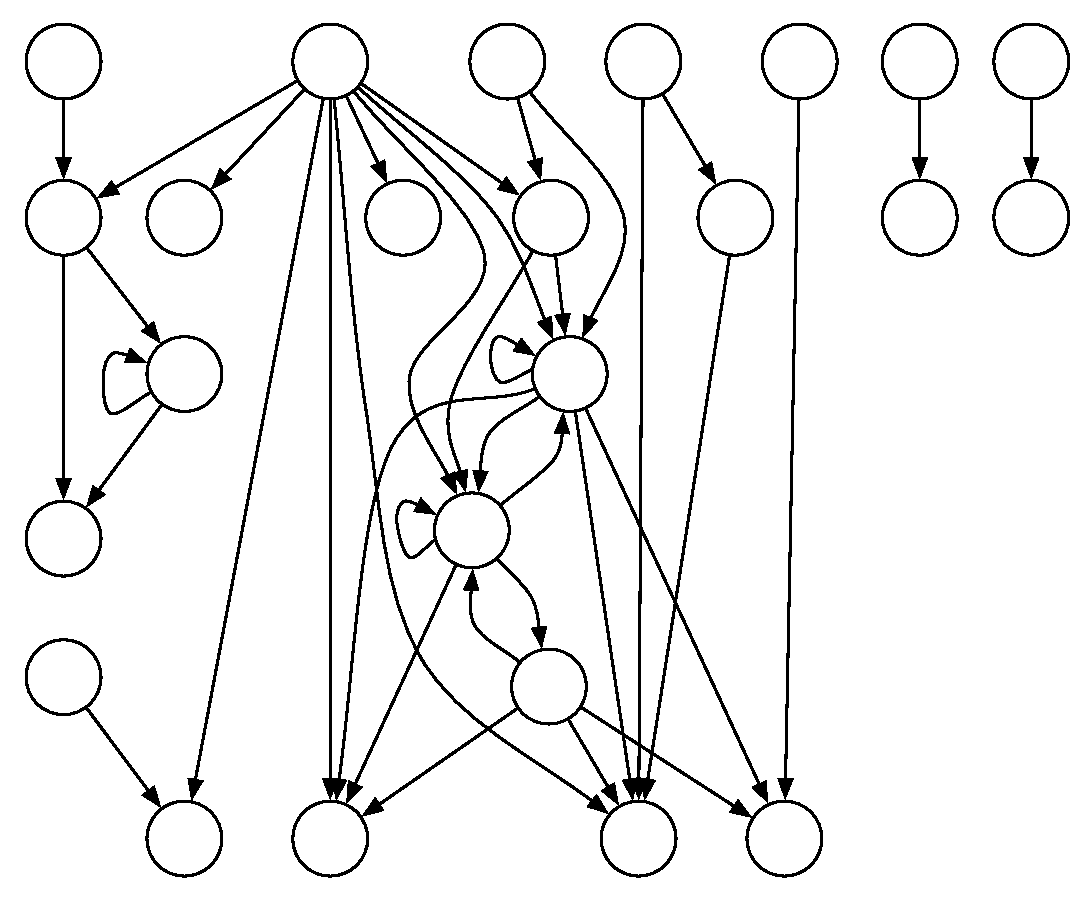
\includegraphics[width=0.47\textwidth]{figs/network}
\label{fig:network}
}
\caption{(a)~Schematic of transcription (top) and translation (bottom).
Here, a transcription factor (TF) binds to DNA close to a gene in a way that
increases gene expression by encouraging RNA polymerase (RNAp) to transcribe
the gene and so produce mRNA.  The mRNA is then translated by ribosomes to
produce sequences of amino acid that ultimately fold into proteins.
Only a small number of transcription factors
directly regulate any gene. Note that a transcription factor's action can also
decrease gene expression. For a more complete picture, see \eg~\cite{Alon:2006}.
(b)~Topology of the transcription network of respiration and redox reactions in
yeast. $X \rightarrow Y$ represents that transcription factor $X$ regulates the
expression of $Y$. Note that this real network has cycles.
Adapted from~\cite{Murray:2011}.}
\end{figure}

We focus on transcription networks, which are a specific class of networks of
interacting genes and proteins that are involved in the production of new
protein. Alon provides an accessible and mathematical introduction to
transcription networks and other biological circuits~\cite{Alon:2006}; below and
in Figure~\ref{fig:biology}, we present a simplified account that motivates this
work. Genes are \emph{transcribed} to produce mRNA, which is then
\emph{translated} into sequences of amino acids that ultimately fold into
proteins.\footnote{In reality, this is a dynamical system where the rates of
production are important. Note that this process need not be linear: a gene (mRNA
transcript) can be transcribed (translated) multiple times, not only in series
but also in parallel fashion.  We also ignore
other \emph{epigenetic} effects, \ie molecular modifications to DNA that do not
change its sequence but alter gene expression,~\eg the addition of methyl groups
to nucleotides in a way that physically blocks transcription.}
In a transcription network, a gene's transcription may be regulated by a set of
proteins called \emph{transcription factors}.
These transcription factors may increase or decrease a gene's transcription by
physically binding to regions of DNA that are typically close to the gene.
In natural systems, only a small number of transcription factors
regulate any single gene, and so transcription networks are sparsely connected.
For example, Balaji~\etal studied a yeast
transcription network of 157 transcription factors regulating 4,410 genes. They
observed this network to have 12,873 interactions (edges) where each gene was
regulated on average by about 2.9 transcription factors, the distribution of
in-degrees was well-described by an exponential fit, and only about 45 genes had
an in-degree of 15 or greater~\cite{Balaji:2006}.

The number of transcription factors varies from hundreds in a bacterium to
thousands in a human cell. Some transcription factors are always present in the
cell and can be thought of as representing a \emph{snapshot} of the
environment~\cite{Alon:2006}.
For example, the presence of sugar molecules in the environment may cause
specific transcription factors to be \emph{activated}, enabling them to regulate
the production of other proteins.  One of these proteins could be an
\emph{end-product}, such as an enzyme that catalyzes a metabolic reaction
involving the sugar. Alternatively, the transcription factor could regulate
another transcription factor that itself
regulates other genes -- we view this as intermediate computation -- and may
participate in further ``computation'' to produce the desired end-result.

While transcription networks may include cycles (loops), here for simplicity we
focus on systems that are directed acyclic graphs, and the resulting computation
can be viewed as a circuit. We illustrate a small, real transcription network in
Figure~\ref{fig:network}. These circuits are by necessity shallow due to
a temporal constraint, that the time required for sufficient quantities of
protein to be produced is of the same order of magnitude as cell-division
time.\footnote{Other kinds of networks, such as signaling networks, operate by
changing the shapes of proteins. The fact that these transformations are rapid
may allow for much larger depth. Note that fast conformational changes govern
how transcription factors directly process information from the environment in
order to regulate gene expression.  In our example, a sugar molecule binds to a
transcription factor and changes its shape in a way that alters its ability to
bind to DNA.} For example, Luscombe~\etal measured the shortest path length (in
number of intermediate nodes) between transcription factors and regulated genes
corresponding to terminal nodes (leaves) in a yeast transcription network. In
the static network, the mean such path length was 4.7 and the longest path
involved 12 intermediate transcription factors~\cite{Luscombe:2004}.

\subsection*{Our Contributions}

First, our contribution is conceptual. We believe that the study of evolvability
from a computational standpoint will benefit by understanding the representation
complexity required to evolve a certain concept class. Motivated by the previous
discussion, in the case of transcription networks, it appears essential that the
representation used be a constant depth and fan-in (boolean or arithmetic)
circuit. Of course, any function that can be represented by such a circuit can
depend only on a constant number of input variables. We ask the
question, when we restrict attention to functions in a given class that depend
only on a constant number of variables, when can evolution succeed?


\subsubsection*{Acknowledgments} 
We would like to thank Leslie Valiant for helpful discussions and comments on an
earlier version of this paper. We are grateful to Frank Solomon for discussing
biological aspects related to this work. VK was supported by a Simons Postdoctoral Fellowship.

\subsubsection*{Related Work}
From the point of view of computer science, there have been very interesting
developments in understanding the power of Valiant's model. We have largely left
these out of this document for reasons of brevity and accessibility. The
interested reader is referred in particular to the work of Vitaly Feldman and
Paul Valiant. The second author's thesis contains an exposition of those
results and other work.

\bibliography{all-refs}
\bibliographystyle{plainnat}

\end{document}
